\chapter{模型/视图 编程}

\section{模型/视图编程简介} 

Qt 中包含了一系列的项目视图类,他们使用了模型/视图架构来管理数据和显示之间的关系。此架构的功能分离特征给开发人员在自定义项目的呈现形式时带来了很大的灵活性,并提供标准的模型接口,以允许将各种数据源与现有项目视图一起使用。在本文档中,我们对模型/视图进行了简要介绍,概述了所涉及的概念,并描述了项目视图系统的结构特征。介绍了体系结构中的每个组件,并给出了示例,这些示例告诉我们如何使用所提供的类。


\section{模型/视图体系架构}

模型-视图-控制器(MVC)是源自 Smalltalk 的设计模式,在构建用户界面时经常使用。在《设计模式》一书中,Gamma 等人写到:


\begin{quote}
MVC 由三种对象组成。模型是应用程序对象,视图是其在屏幕上的呈现,控制器定义了用户界面对用户输入的反应方式。 在MVC之前,用户界面设计往往会将这些对象整合在一起。 MVC 使它们解耦以增加灵活性和重用性。	
\end{quote}

如果将视图和控制器对象组合在一起,就是模型/视图架构。基于将数据的存储方式与向用户呈现的方式分开的原理,模型/视图架构提供了一个更简单的框架。这种分离使得可以在几个不同的视图中显示相同的数据,并实现新的视图类型,而无需更改基础数据结构。为了灵活处理用户输入,我们引入了委托的概念。在此框架中使用委托的好处在于,它允许自定义呈现和编辑数据项的方式。

%\begin{tabular}{|l|p{25em}|}
%\hline
%    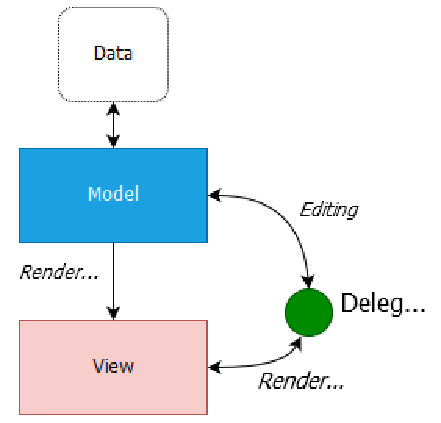
\includegraphics[width=0.4\textwidth,keepaspectratio]{Model_View_architecture.pdf}
%  & 模型/视图架构 模型与数据源通信,为架构中的其他组件提供接口。通信的性质取决于数据源的类型以及模型的实现方式。
%
%
%视图从模型中获取模型索引; 这些索引是对数据项的引用。 通过向模型提供模型索引,视图可以从数据源检索出数据项。
%
%
%在标准视图中,委托负责渲染显示数据项。 当编辑项目后,委托将直接通过模型索引与模型进行通信。\\
%
%\hline	
%\end{tabular}


\begin{tabular}{|l|m{25em}|}
\hline
   
    
    \adjustbox{valign=t}{ 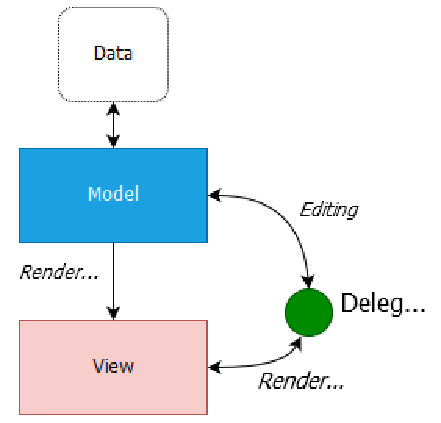
\includegraphics[width=0.4\textwidth]{Model_View_architecture.pdf}}
  & 模型/视图架构 模型与数据源通信,为架构中的其他组件提供接口。通信的性质取决于数据源的类型以及模型的实现方式。


视图从模型中获取模型索引; 这些索引是对数据项的引用。 通过向模型提供模型索引,视图可以从数据源检索出数据项。


在标准视图中,委托负责渲染显示数据项。 当编辑项目后,委托将直接通过模型索引与模型进行通信。\\

\hline	
\end{tabular}


通常,模型/视图类可以分为上述三个组:模型,视图和委托。这些组件中的每个组件都由抽象类定义,这些抽象类提供了公共接口,并在某些情况下提供了一些功能的默认实现。抽象类应被子类化,以提供其他组件期望的全部功能;当然也可以编写专用组件。

模型、视图和委托之间通过信号槽通信。

\begin{compactitem}[\arr]
\item 数据源的数据发生改变时模型将发射信号通知视图。
\item 用户交互发生改变时,视图将发射相应的信号。
\item 在编辑期间,委托将发射信号来告知模型和视图有关编辑器的状态。
\end{compactitem}


\section{模型}

所有项目模型均基于 QAbstractItemModel 类。此类定义一个接口,视图和委托使用该接口访问数据。数据本身不必存储在模型中。它可以保存在由单独的类,文件,数据库或某些其他应用程序组件提供的数据结构或存储库中。


有关模型的基本概念在 “模型类”部分中介绍。


QAbstractItemModel 提供了一个数据接口,该接口足够灵活,可以处理以表,列表和树的形式表示数据的视图。但是,当为列表和类似表的数据结构实现新模型时,QAbstractListModel 和 QAbstractTableModel 类是更好的选择,因为它们提供了常用功能的默认实现。这些类中的每一个都可以被子类化以提供支持特殊类型的列表和表的模型。


在 创建新模型 部分中讨论了模型子类化的过程。


Qt提供了一些现成的模型,可用于处理数据项:

\begin{compactitem}[\arr]
\item QStringListModel 用于存储一列简单的 QString 类型的项目。
\item QStandardItemModel 用于管理更复杂的树形结构项目,每个项目可以包含任意数据。
\item QFileSystemModel 提供有关本地归档系统中文件和目录的信息。
\item QSqlQueryModel,QSqlTableModel 和 QSqlRelationalTableModel 用于在使用模型/视图架构时访问数据库。
\end{compactitem}


如果这些标准模型不满足您的要求,则可以将 QAbstractItemModel,QAbstractListModel 或 QAbstractTableModel 子类化以创建您自己的自定义模型。

\section{视图}

Qt 提供了针对各种视图的完整实现:QListView 用于显示项目列表,QTableView 用于显示表结构模型的数据,QTreeView 在一个分层次的结构列表中显示数据项。这些类均基于 QAbstractItemView 抽象基类。尽管这些类都是已经实现好的,但也可以将它们子类化以提供满足我们需求的自定义视图。


所有可用的视图可在 视图类 部分中进行查阅。

\section{委托}

QAbstractItemDelegate 是模型/视图框架中委托的抽象基类。默认委托实现由 QStyledItemDelegate 提供, Qt 中的标准视图都将其作为默认委托。但是,QStyledItemDelegate 和 QItemDelegate 是绘制和为视图中的项目提供编辑器的独立替代方法。它们之间的区别在于 QStyledItemDelegate 使用当前样式来绘制其项目。因此,在实现自定义委托或使用 Qt 样式表时,建议将 QStyledItemDelegate 用作基类。


委托在 “委托类” 部分中进行了描述。

\section{排序}

在模型/视图架构中,有两种方法可以进行排序;选择哪种方法取决于底层使用的模型。


如果您的模型是可排序的,即重新实现 QAbstractItemModel::sort() 函数,则 QTableView 和 QTreeView 都提供了API,可让您以编程方式对模型数据进行排序。 另外,通过将 QHeaderView::sortIndicatorChanged() 信号连接到 QTableView::sortByColumn() 槽函数或 QTreeView::sortByColumn() 槽函数,可以启用交互式排序(即允许用户通过单击视图的标题对数据进行排序))。


如果您的模型没有所需的接口,或者如果您想使用列表视图来呈现数据,则另一种方法是在视图呈现数据之前,使用委托模型来转换模型的结构。 有关 代理模型 的部分将对此进行详细介绍。

\section{便捷类}

从标准视图类派生出了许多便捷类,用于 Qt 中基于项目的项目视图类和表类,它们不打算被子类化。

比如 QListWidget,QTreeWidget 和 QTableWidget。

这些类的灵活性不如视图类,并且不能与任意模型一起使用。我们建议您使用模型/视图方法来处理项目视图中的数据,除非您强烈需要一组基于项目的类。

如果希望在使用基于项目的接口的同时利用模型/视图方法提供的功能,请考虑将视图类(例如 QListView,QTableView 和 QTreeView )与 QStandardItemModel 一起使用。

\section{使用模型和视图}

以下各节说明如何在 Qt 中使用模型/视图模型。每个部分都包含一个示例,紧接着是展示如何创建新组件。

\subsection{Qt 中包含的两个模型}

Qt 提供的两个标准模型是 QStandardItemModel 和 QFileSystemModel。QStandardItemModel 是一个多功能模型,可用于表示列表,表和树视图所需的各种不同的数据结构。该模型还保存数据项。QFileSystemModel 是用于维护有关目录内容的信息的模型,它本身不保存任何数据项,而仅表示本地文件系统上的文件和目录。

QFileSystemModel 提供了一个现成的模型用来测试使用,并且可以通过简单的配置就可以使用现有的数据。使用该模型,我们可以展示如何创建一个可用于现成视图的模型,并探索如何使用模型索引来操控数据。

\subsection{通过现有模型使用视图}

QListView 和 QTreeView 类是最适合与 QFileSystemModel一起使用的视图。下面提供的示例是分别在树形视图和列表视图中显示相同的目录内容。这些视图共享用户的选择,以便在两个视图中突出显示所选的项目。

\begin{figure}[hpt!]  
	\centering
    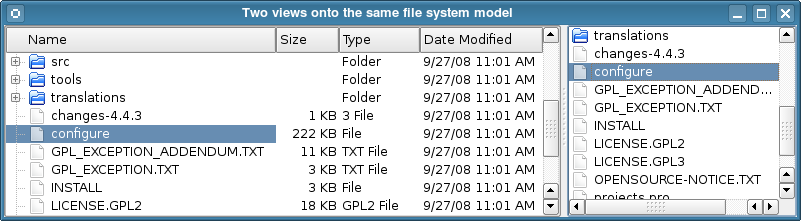
\includegraphics[width=0.5\textwidth]{shareddirmodel}
\end{figure}

我们使用了现成的模型 QFileSystemModel,并创建了一些视图来显示目录的内容。展示了使用模型的最简单方法。 该模型的构建和使用是在单个 main() 函数中执行的:

\begin{lstlisting}[language=C++]
int main(int argc, char *argv[])
{
    QApplication app(argc, argv);
    QSplitter *splitter = new QSplitter;

    QFileSystemModel *model = new QFileSystemModel;
    model->setRootPath(QDir::currentPath());
\end{lstlisting}

该模型被设置为使用来自特定文件系统的数据。调用 setRootPath() 将告诉模型文件系统上的哪个驱动器会暴露给视图。

我们使用同一个模型创建两个不同的视图,来查看模型中的项目呈现出来的效果:

\begin{lstlisting}[language=C++]
QTreeView *tree = new QTreeView(splitter);
tree->setModel(model);
tree->setRootIndex(model->index(QDir::currentPath()));

QListView *list = new QListView(splitter);
list->setModel(model);
list->setRootIndex(model->index(QDir::currentPath()));
\end{lstlisting}

视图的构造方法与其他部件一样。设置视图来显示模型中的项目仅需使用目录模型作为参数来调用视图的 setModel() 函数即可。我们通过在每个视图上调用 setRootIndex() 函数来过滤模型提供的数据,并从文件系统模型中为当前目录传递合适的模型索引。

这种情况下对于 QFileSystemModel 来说只能通过传递一个目录参数来使用 index() 函数获取索引,模型索引在 模型类 部分中讨论。

该函数的其余部分是在分裂器部件中显示视图,并运行应用程序的事件循环:

\begin{lstlisting}[language=C++]
    splitter->setWindowTitle("Two views onto the same file system model");
    splitter->show();
    return app.exec();
}
\end{lstlisting}

在上面的示例中,我们忽略了如何处理项目选择。 在 处理项目视图中的选择项 部分中将更详细地介绍。

\section{模型类}

在学习如何处理选择项之前,理解模型/视图框架中使用的概念是很有用的。

\subsection{基本概念}

在模型/视图体系结构中,模型提供了视图和委托用来访问数据的标准接口。在 Qt 中,标准接口由 QAbstractItemModel 类定义。无论数据项如何存储在任何基础数据结构中,QAbstractItemModel 的所有子类都将数据表示为一个有层次的包含项表的结构。视图使用此约定来访问模型中的数据项,但是它们向用户呈现此信息的方式不受限制。

\begin{figure}[hpt!]  
	\centering
    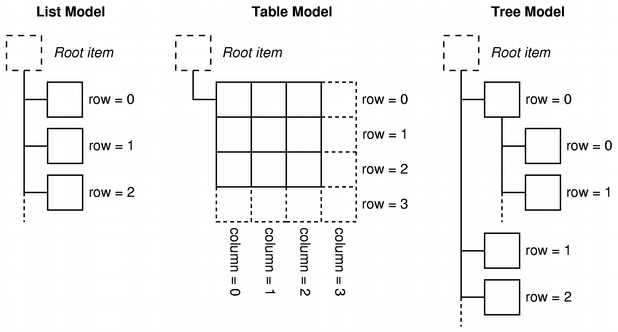
\includegraphics[width=0.5\textwidth]{modelview-models}
\end{figure}

模型通过信号槽机制通知所有附加视图有关数据更改的信息。

本节描述一些基本概念,这些概念对于其他组件通过模型类访问数据项的方式至关重要。 稍后的部分将讨论更高级的概念。

\section{模型索引}

为了确保数据的表示方式与访问方式分开,引入了模型索引的概念。通过模型获得的每条信息都由模型索引表示。视图和委托使用这些索引来请求要显示的数据项。

所以,只有模型需要知道如何获取数据和定义数据类型。模型索引包含一个指向创建它们的模型的指针,以免在使用多个模型时造成混淆。

\begin{lstlisting}[language=C++]
QAbstractItemModel *model = index.model();
\end{lstlisting}

模型索引提供了一个对信息的临时的引用,可用于通过模型检索或修改数据。由于模型可能会不时重组其内部结构,因此模型索引可能会变得无效,不应进行存储。如果需要长期使用一条信息,则必须创建一个持久的模型索引。这为模型保持最新状态提供了参考。临时模型索引由 QModelIndex 类提供,而持久模型索引由 QPersistentModelIndex 类提供。

要获得与数据项相对应的模型索引,必须为模型指定三个属性:行号,列号和父项的模型索引。以下各节将详细描述和解释这些属性。

\section{行和列}

在基本的形式中,可以将模型作为一个简单的表进行访问,项目按行和列的编号位于其中。

这并不意味着底层数据存储在数组结构中;行号和列号的使用仅仅是组件之间相互通信的约定。

我们可以通过在模型中指定给定项目的行号和列号来检索有关任何给定项目的信息,我们接收到的是代表该项目的索引:

\begin{lstlisting}[language=C++]
QModelIndex index = model->index(row, column, ...);
\end{lstlisting}


为简单的单层数据结构(例如列表和表)提供接口的模型不需要提供任何其他信息,但是,如上述代码所示,在获取模型索引时,我们需要提供更多信息。

\begin{tabular}{|l|m{25em}|}
\hline
\adjustbox{valign=t}{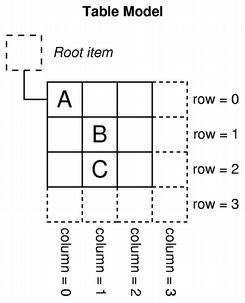
\includegraphics[width=0.5\textwidth]{modelview-tablemodel}}
  & 
  行和列
  
该图显示了基本表模型的表示形式,其中每个项目都由一对行号和列号定位。通过将相关的行号和列号传递给模型,我们获得了一个引用数据项的模型索引。

\begin{lstlisting}[language=C++]
QModelIndex indexA = model->index(0, 0, QModelIndex());
QModelIndex indexB = model->index(1, 1, QModelIndex());
QModelIndex indexC = model->index(2, 1, QModelIndex());
\end{lstlisting}

始终通过用 QModelIndex() 指定为其父项来引用模型中的顶级项目。下一节将对此进行讨论。\\
\hline	
\end{tabular}

\section{项的父项}
当在表视图或列表视图中使用数据时,模型提供的类似于表的接口就非常合适。行号和列号系统准确地映射到视图显示项目的方式上。但是,诸如树状视图的结构对于模型项目的操作要求模型提供更灵活的接口。每个项目也可以是另一个项目表的父项,就像树状视图中的顶级项目可以包含另一个项目列表一样。

当请求模型项的索引时,我们必须提供有关该项父项的一些信息。在模型之外,引用项目的唯一方法是通过模型索引,因此还必须提供父模型索引:

\begin{lstlisting}[language=C++]
QModelIndex index = model->index(row, column, parent);
\end{lstlisting}

\begin{tabular}{|l|m{25em}|}
\hline
    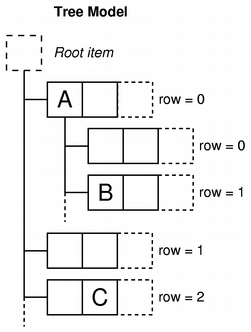
\includegraphics[width=0.5\textwidth]{modelview-treemodel}
  & 
父项、行和列

该图展示了树模型的表示形式,其中每一项均由父项、行号和列号检索出来。

“A”和“C”项在模型中为同级顶级:

\begin{lstlisting}[language=C++]
QModelIndex indexA = model->index(0, 0, QModelIndex());
QModelIndex indexC = model->index(2, 1, QModelIndex());
\end{lstlisting}

“A”项有多个子项。使用以下代码获得“B”项的模型索引:

\begin{lstlisting}[language=C++]
QModelIndex indexB = model->index(1, 0, indexA);
\end{lstlisting}
\\
\hline	
\end{tabular}

\section{项角色}

模型中的项可以为其他组件扮演各种不同的角色,从而可以为不同的数据提供不同的方案。 例如,Qt::DisplayRole 用于访问可以在视图中显示为文本的字符串。通常,项包含许多不同角色的数据,标准角色由 Qt::ItemDataRole 定义。

我们可以通过向模型传递与该项相对应的模型索引,并指定一个角色来获取所需的数据类型,从而获得我们想要的数据:

\begin{lstlisting}[language=C++]
QVariant value = model->data(index, role);
\end{lstlisting}


\begin{tabular}{|l|m{25em}|}
\hline
    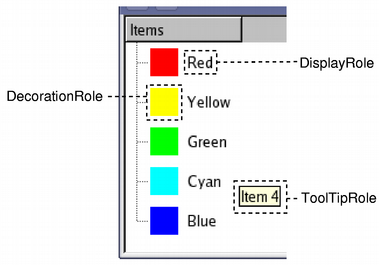
\includegraphics[width=0.5\textwidth]{modelview-roles}
  & 
项角色

项角色向模型指示要引用的数据类型。视图可以以不同的方式显示角色,因此为每个角色提供适当的信息很重要。

创建新模型 部分将更详细地介绍角色的某些特定用法。\\
\hline	
\end{tabular}


项标准角色 Qt::ItemDataRole 涵盖了大部分常用的项角色。通过为每个角色提供适当的项目数据,模型可以向视图和委托提示如何将项呈现给用户。不同类型的视图可以根据自身需要解释或忽略此信息。也可以为特定目的定义其他角色。

\section{摘要}

\begin{compactitem}[\arr]
\item 模型索引以独立于任何底层数据结构的方式提供给视图和委托有关模型所提供项的位置的信息。
\item 项通过其行号和列号以及其父项的模型索引检索出来。
\item 模型索引是由模型根据其他组件(例如视图和委托)的请求构造出来的。
\item 如果使用 index() 请求索引时为父项指定了有效的模型索引,则返回的索引将引用模型中该父项之下的项。获得的索引指向该项目的子项。
\item 如果使用 index() 请求索引时为父项指定了无效的模型索引,则返回的索引引用模型中的顶级项。
\item 项角色 用来区分与项关联的不同类型的数据。
\end{compactitem}

\section{使用模型索引}

为了演示如何使用模型索引从模型中检索数据,我们设置了一个没有视图的 QFileSystemModel,并在部件中显示文件和目录的名称。尽管这没有展示使用模型的正常方法,但是它说明了在处理模型索引时模型使用的规则。

QFileSystemModel 加载是异步的,以最大程度地减少系统资源的使用。在处理此模型时,我们必须考虑到这一点。

我们通过以下方式构造文件系统模型:

\begin{lstlisting}[language=C++]
QFileSystemModel *model = new QFileSystemModel;
connect(model, &QFileSystemModel::directoryLoaded, [model](const QString &directory) {
    QModelIndex parentIndex = model->index(directory);
    int numRows = model->rowCount(parentIndex);
});
model->setRootPath(QDir::currentPath);
\end{lstlisting}

在这种情况下,我们首先设置默认的 QFileSystemModel 。我们将其连接到 \hl{lambda},在其中我们将使用该模型提供的 index() 的特定实现来获取父索引。 在 \hl{lambda} 中,我们使用 rowCount() 函数计算模型中的行数。最后,我们设 QFileSystemModel 的根路径,以便它开始加载数据并触发 \hl{lambda} 。

为简单起见,我们只处理模型第一栏中的项目。我们依次检查每一行,获取每一行中第一项的模型索引,然后读取模型中为该项存储的数据。

\begin{lstlisting}[language=C++]
for (int row = 0; row < numRows; ++row) {
    QModelIndex index = model->index(row, 0, parentIndex);
\end{lstlisting}

为了获得模型索引,我们指定行号,列号(第一列为零),并为所需的所有项的父项指定适当的模型索引。使用模型的 data() 函数检索存储在每个项目中的文本。我们指定模型索引和 DisplayRole 获取字符串形式的项数据。

\begin{lstlisting}[language=C++]
QString text = model->data(index, Qt::DisplayRole).toString();
    // Display the text in a widget.

}
\end{lstlisting}

以上示例演示了从模型中检索数据的基本用法:

\begin{compactitem}[\arr]
\item 模型的大小范围可以使用 rowCount() 和 columnCount 获取到。这些函数通常需要指定一个父项模型索引。
\item 模型索引用于访问模型中的数据项。指定一个项需要行、列和父项的模型索引。
\item 通过 \hl{QModelIndex()} 指定一个空的父项的索引来访问模型中的顶层项。
\item 项包含不同角色的数据。要获得特定角色的数据,必须同时向模型提供模型索引和角色。
\end{compactitem}


\subsection{拓展阅读}

可以通过提供了标准接口的 QAbstractItemModel 类来创建新模型。在 创建新模型 部分,我们将通过创建一个方便可用的保存字符串列表的模型来展示这一点。

\section{视图类}
\subsection{概念}

在模型/视图架构中,视图从模型中获取数据项并将其呈现给用户。呈现数据的方式不必类似于模型提供数据的方式,而可以与用于存储数据项的底层数据结构完全不同。

通过使用 QAbstractItemModel 提供的标准模型接口,QAbstractItemView 提供的标准视图接口以及使用表示数据项的模型索引来实现内容和表示的分离。视图通常管理从模型获得的数据的整体布局。它们可以自己呈现单个数据项,或使用委托来处理渲染和编辑功能。

除了显示数据外,视图还处理项目之间的导航以及项目选择。这些视图还实现了基本的用户界面功能,例如上下文菜单和拖放功能。视图可以提供项目的默认编辑功能,也可以与 委托 一起使用以提供自定义编辑器。

可以在没有模型的情况下构造视图,但是必须提供模型才能显示有用的信息。视图通过使用 选择项 来跟踪用户选择的项目,这些选择项可以被每个视图单独维护,或者在多个视图之间共享。

一些视图,例如 QTableView 和 QTreeView,需要显示表头和项目。这些由视图类 QHeaderView 实现。表头通常与包含它们的视图访问的是同一个模型。他们使用 QAbstractItemModel::headerData() 函数从模型中检索数据,并且通常以标签形式显示表头信息。可以继承 QHeaderView 类实现新的标头,以为视图提供更专业的标签。

